\minitoc
This appendix is organized into three sections. It begins by delving into the TensorFlow Lite delegate interface implementation for the \gls{tp} and its associated hardware drivers. Following this, modifications made to the TensorFlow Lite library are highlighted. The appendix concludes with a detailed presentation of the \gls{sbs} algorithm.
%%%%%%%%%%%%%%%%%%%%%%%%%%%%%%%%%%%%%%%%%%%%%%%%%%%%%%%%%%%%%%%%%%
\section{Tensor Processor Delegate and Hardware Drivers}
\label{chap:appendix_delegate}
This section provides an overview of the directory structure and key components involved in the development of \gls{tp} delegate and hardware drivers. The organized layout of these sections aids in understanding the architecture and implementation.

The diagram in \Fig{fig:sw_tp_delegate_diagram_appendix} provides a comprehensive overview of the \gls{tp} delegate and hardware drivers, presenting the interactions among classes and showing both their public and private functions. The subsequent subsections provide the directory structure for the implemented classes.

\begin{figure}[h!]
	\centering
	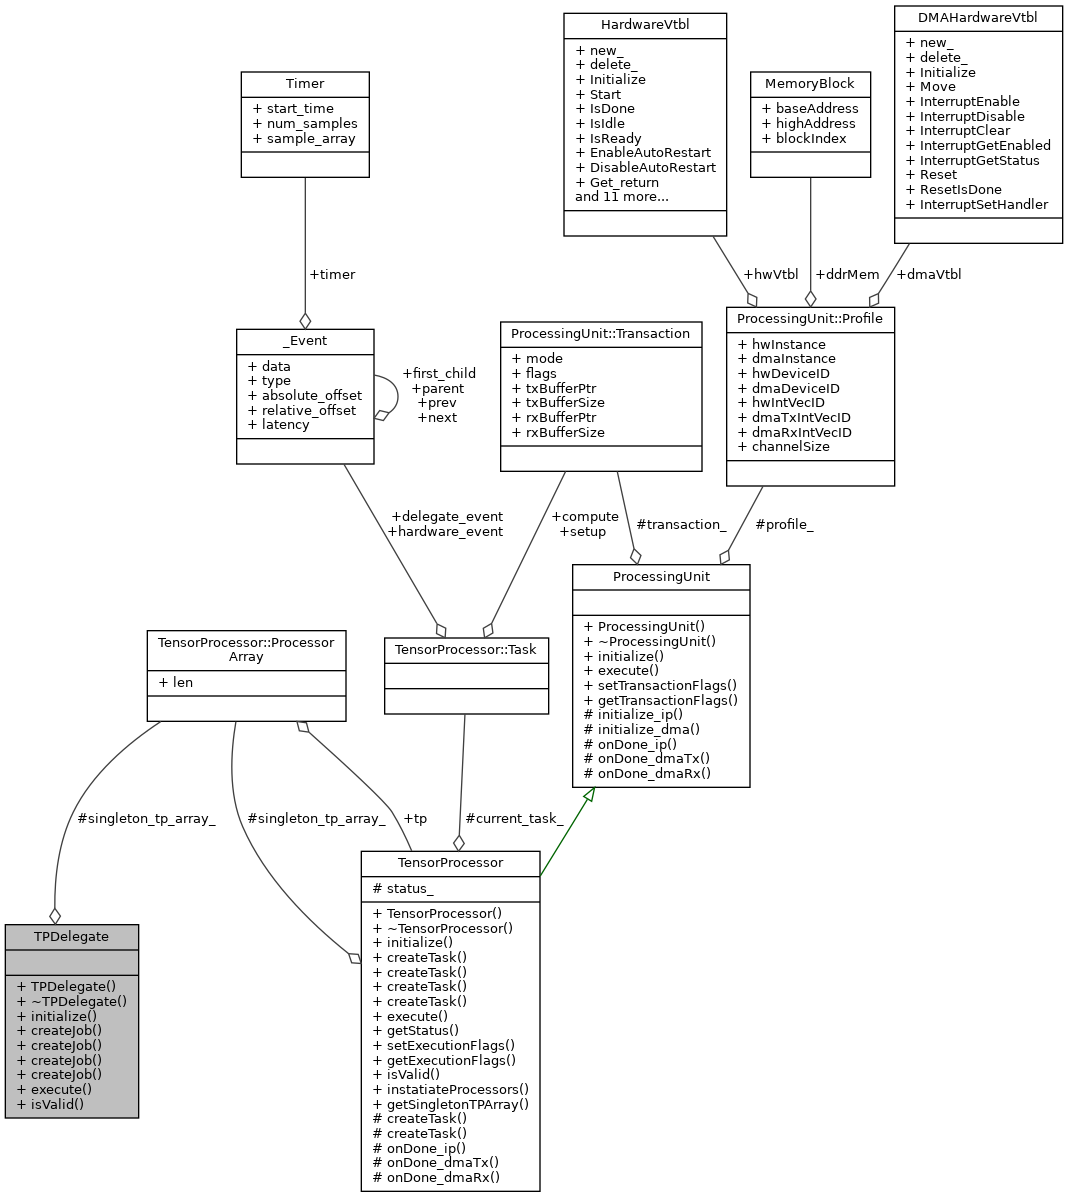
\includegraphics[width=\textwidth]{./figures/class_t_p_delegate__coll__graph.png}
	\caption{Collaboration diagram of the \gls{tp} delegate and hardware drivers.}
	\label{fig:sw_tp_delegate_diagram_appendix}
\end{figure}

This implementation is available to the community as an open-source project at:

\url{https://github.com/YaribNevarez/tensorflow-lite-fpga-delegate.git}

\FloatBarrier

\subsection {Tensor Processor Delegate}
The \textit{TPDelegate} class serves as the intermediary between the \gls{ml} library and the hardware drivers. It facilitates hardware initialization, creates computational \textit{Jobs} for tensor operations such as \textit{Conv2D} and \textit{DepthwiseConv2D} in both floating-point and fixed-point formats, and provides the means to execute these \textit{Jobs}. TensorFlow Lite invokes these functions to delegate the computational load to the \gls{tp}.

Serving a dual role, the \textit{TPDelegate} acts as a container for multiple \textit{TensorProcessor} object instances, containing an internal array of these. For horizontal scalability, the \textit{TPDelegate} can manage multiple \textit{TensorProcessor} instances. Meanwhile, the \textit{TensorProcessor} class, inheriting from the \textit{ProcessingUnit} class (hardware driver), encapsulates hardware interactions and offers a bridge interface to them.

The \gls{tp} delegate module is composed of the following directory structure:

\begin{figure}[!h]
\dirtree{%
	.1 libs/.
	.2 delegates/.
	.3 inc/.
	.4 tensor\_processor.h.
	.4 tp\_delegate.h.
	.3 src/.
	.4 tensor\_processor.cpp.
	.4 tp\_delegate.cpp.
}
\end{figure}
\FloatBarrier

\subsection {Hardware Drivers}
The driver module integrates the \textit{ProcessingUnit} class and virtual function tables specifically designed for low-level handling of the \gls{tp} and \gls{dma}. The \textit{ProcessingUnit} class encapsulates the hardware interactions, including initialization, execution, cache memory coherence, and interrupt handling, by employing the hardware virtual tables. The virtual function tables act as wrappers for hardware functions, facilitating the smooth transition or interchange of hardware components.

The hardware drivers module is structured as follows, including source files and headers:
\begin{figure}[!h]
	\dirtree{%
	.1 libs/.
	.2 drivers/.
	.3 inc/.
	.4 conv\_vtbl.h.
	.4 dma\_vtbl.h.
	.4 processing\_unit.h.
	.3 src/.
	.4 conv\_vtbl.c.
	.4 dma\_vtbl.c.
	.4 processing\_unit.cpp.
}
\end{figure}
\FloatBarrier


\subsection {ARM Generic Interrupt Controller}
The \gls{gic} orchestrates interrupts within multiple core \gls{soc}. The \gls{gic} ensures interrupt requests from diverse peripherals are prioritized and channeled to the suitable processor core inside the \gls{soc}. This module serves as a wrapper tailored for the Xilinx \gls{gic}, which is used by the hardware drivers. This wrapper facilitates the smooth transition or interchange of \gls{soc} types and brands.

The \gls{gic} module is composed of the following directory structure:
\begin{figure}[!h]
	\dirtree{%
		.1 libs/.
		.2 arm/.
		.3 inc/.
		.4 gic.h.
		.3 src/.
		.4 gic.c.
	}
\end{figure}
\FloatBarrier

\subsection {Supporting Classes}
The supporting classes offer foundational utilities that enhance various modules through a structured set of functionalities. These provide macros for decomposing \gls{fp} values into their sign, exponent, and mantissa, offering more granular control over numerical representations. This module also provides memory management tailored for embedded devices, ensuring optimal memory allocation while considering the constraints of the system. Additionally, \textit{Event} and \textit{Timer} classes enhance performance monitoring by logging events and measuring timings with a hardware timer, facilitating a profound understanding of system performance.

The supporting classes comprises utility classes and their corresponding source files:
\begin{figure}[!h]
	\dirtree{%
		.1 libs/.
		.2 utilities/.
		.3 inc/.
		.4 custom\_float.h.
		.4 event.h.
		.4 memory\_manager.h.
		.4 miscellaneous.h.
		.4 timer.h.
		.3 src/.
		.4 event.c.
		.4 memory\_manager.c.
		.4 miscellaneous.c.
		.4 timer.c.
	}
\end{figure}
\FloatBarrier

\section{TensorFlow Lite Integration}
\label{chap:code_changes}
This appendix subsection details the modifications made to the TensorFlow Lite library to incorporate the delegate interface designed for the proposed \gls{tp}. This begins by showcasing a directory tree that highlights the altered source and header files. Following this, it is presented the specific code changes in each file.

\begin{figure}[!h]

	\dirtree{%
		.1 tensorflow/.
		.2 lite/.
		.3 c/.
		.4 common.h.
		.4 \vdots.
		.3 micro/.
		.4 kernels/.
		.5 conv.cpp.
		.5 depthwise\_conv.cpp.
		.5 kernel\_util.cpp.
		.5 kernel\_util.h.
		.5 \vdots.
		.4 micro\_graph.cpp.
		.4 micro\_graph.h.
		.4 micro\_interpreter.cpp.
		.4 micro\_interpreter.h.
		.4 \vdots.
	}
\end{figure}
\FloatBarrier

\subsection*{common.h}

This file defines the data types employed within the TensorFlow Lite library, including compute nodes, tensors, quantization types, delegates, and the execution context. Within the execution context structure, the \textit{GetDelegate()} function pointer has been introduced to access to the custom delegate instance during execution.

\begin{verbatim}
typedef struct TfLiteContext {
  // ...
  void * (*GetDelegate) (const struct TfLiteContext* context);
} TfLiteContext;
\end{verbatim}

\subsection*{conv.cpp}
This file contains the \textit{Conv2D} tensor operator. Within it, the allocation and initialization of the Job instance have been incorporated. This instance carries the essential parameters required to execute this tensor operation on the \gls{tp} via the delegate. The Job object is instantiated based on the tensor data type, whether it is floating-point or fixed-point. For a more generic \gls{tp}, this mechanism would be positioned at a higher level to circumvent direct modifications to specific tensor operator modules.

\begin{verbatim}
#include "tp_delegate.h"
// ...
void* Init(TfLiteContext* context, const char* buffer, size_t length)
{
  // ...
  return context->AllocatePersistentBuffer (context, 
    sizeof(OpDataConv) + sizeof(TPDelegate::Job));
}
\end{verbatim}

\begin{verbatim}
TfLiteStatus Eval(TfLiteContext* context, TfLiteNode* node)
{
  TPDelegate * delegate = reinterpret_cast<TPDelegate *>
    (tflite::micro::GetDelegate (context));
  // ...
  TPDelegate::Job & job = *(reinterpret_cast<TPDelegate::Job*>
    (node->user_data + sizeof(OpDataConv)));
  // ...
  
  if (delegate != nullptr)
  {
    switch (input->type)
    {
      case kTfLiteFloat32:
      {
        if (!TPDelegate::isValid (job))
        {
          job = delegate->createJob(ConvParamsFloat (params, data),
            tflite::micro::GetTensorShape (input),
            tflite::micro::GetTensorData<float> (input),
            tflite::micro::GetTensorShape (filter),
            tflite::micro::GetTensorData<float> (filter),
            tflite::micro::GetTensorShape (bias),
            tflite::micro::GetTensorData<float> (bias),
            tflite::micro::GetTensorShape (output),
            tflite::micro::GetTensorData<float> (output),
            reinterpret_cast<Event *> (node->delegate));
        }
        delegate->execute (job);
        break;
      }
      case kTfLiteInt8:
      {
        if (!TPDelegate::isValid (job))
        {
          job = delegate->createJob(
            ConvParamsQuantized (params, data),
            data.per_channel_output_multiplier,
            data.per_channel_output_shift,
            tflite::micro::GetTensorShape (input),
            tflite::micro::GetTensorData<int8_t> (input),
            tflite::micro::GetTensorShape (filter),
            tflite::micro::GetTensorData<int8_t> (filter),
            tflite::micro::GetTensorShape (bias),
            tflite::micro::GetTensorData<int32_t> (bias),
            tflite::micro::GetTensorShape (output),
            tflite::micro::GetTensorData<int8_t> (output),
            reinterpret_cast<Event *> (node->delegate));
        }
        delegate->execute (job);
        break;
      }
      default:
        TF_LITE_KERNEL_LOG(context, "Type %s (%d) not supported.",
          TfLiteTypeGetName (input->type), input->type);
        return kTfLiteError;
    }
  }
  else
  {
    // ...
  }
// ...
\end{verbatim}

\subsection*{depthwise\_conv.cpp}

This file contains the \textit{DepthwiseConv2D} tensor operator. Within it, the allocation and initialization of the Job instance have been incorporated. This instance carries the essential parameters required to execute this tensor operation on the \gls{tp} via the delegate. The Job object is instantiated based on the tensor data type, whether it is floating-point or fixed-point. For a more generic \gls{tp}, this mechanism would be positioned at a higher level to circumvent direct modifications to specific tensor operator modules.

\begin{verbatim}
#include "tp_delegate.h"
// ...
void* Init(TfLiteContext* context, const char* buffer, size_t length)
{
  // ...
  return context->AllocatePersistentBuffer (context,
    sizeof(OpDataConv) + sizeof(TPDelegate::Job));
}
\end{verbatim}

\begin{verbatim}
TfLiteStatus Eval(TfLiteContext* context, TfLiteNode* node)
{
  TPDelegate * delegate = reinterpret_cast<TPDelegate *>
    (tflite::micro::GetDelegate (context));
  // ...
  TPDelegate::Job & job = *(reinterpret_cast<TPDelegate::Job*>
    (node->user_data + sizeof(OpDataConv)));
  // ...

  if (delegate != nullptr)
  {
    switch (input->type)
    {
      case kTfLiteFloat32:
      {
        if (!TPDelegate::isValid (job))
        {
          job = delegate->createJob(ConvParamsFloat (params, data),
            tflite::micro::GetTensorShape (input),
            tflite::micro::GetTensorData<float> (input),
            tflite::micro::GetTensorShape (filter),
            tflite::micro::GetTensorData<float> (filter),
            tflite::micro::GetTensorShape (bias),
            tflite::micro::GetTensorData<float> (bias),
            tflite::micro::GetTensorShape (output),
            tflite::micro::GetTensorData<float> (output),
            reinterpret_cast<Event *> (node->delegate));
        }
        delegate->execute (job);
        break;
      }
      case kTfLiteInt8:
      {
        if (!TPDelegate::isValid (job))
        {
          job = delegate->createJob(
            ConvParamsQuantized (params, data),
            data.per_channel_output_multiplier,
            data.per_channel_output_shift,
            tflite::micro::GetTensorShape (input),
            tflite::micro::GetTensorData<int8_t> (input),
            tflite::micro::GetTensorShape (filter),
            tflite::micro::GetTensorData<int8_t> (filter),
            tflite::micro::GetTensorShape (bias),
            tflite::micro::GetTensorData<int32_t> (bias),
            tflite::micro::GetTensorShape (output),
            tflite::micro::GetTensorData<int8_t> (output),
            reinterpret_cast<Event *> (node->delegate));
        }
        delegate->execute (job);
        break;
      }
      default:
        TF_LITE_KERNEL_LOG(context, "Type %s (%d) not supported.",
          TfLiteTypeGetName (input->type), input->type);
        return kTfLiteError;
    }
  }
  else
  {
    // ...
  }
// ...
\end{verbatim}

\subsection*{kernel\_util.cpp}
This source file contains utility functions employed by the kernels or tensor operators during execution. Within this file, a wrapper function has been added to retrieve the delegate instance from the execution context.

\begin{verbatim}
// ...
void * GetDelegate (const TfLiteContext* context)
{
  TFLITE_DCHECK(context != nullptr);
  return context->GetDelegate (context);
}
\end{verbatim}

\subsection*{kernel\_util.h}
This header file outlines the prototypes of utility functions used by the kernels or tensor operators during execution. It is added the prototype for the wrapper function designed to extract the delegate instance from the execution context.
\begin{verbatim}
// ...
void* GetDelegate (const TfLiteContext* context);
\end{verbatim}

\subsection*{micro\_graph.cpp}
This source file contains the code associated with traversing and execution of the computational graph or model. It incorporates functions for the allocation, initialization, preparation, execution, and disposal of the model graph. An event logger has been introduced to this class, logging each compute node activity, offering detailed timing data for performance analysis.
\begin{verbatim}
#include "event.h"
// ...
MicroGraph::~MicroGraph ()
{
  DisposeEventLogger ();
}
// ...
TfLiteStatus MicroGraph::InvokeSubgraph(int subgraph_idx)
{
  // ...
  for (size_t i = 0; i < subgraph->operators()->size(); ++i)
  {
    // ...
    Event_start (reinterpret_cast<Event*> (event_array_[i]));
    
    TFLITE_DCHECK(registration->invoke);
    TfLiteStatus invoke_status = registration->invoke(context_, node);
    
    Event_stop (reinterpret_cast<Event*> (event_array_[i]));
    // ...
  }
  // ...
}
// ...
void MicroGraph::AllocateEventLogger (void * parent, int subgraph_idx)
{
  if (event_array_ == nullptr && subgraph_allocations_ != nullptr)
  {
    const SubGraph* subgraph = (*subgraphs_)[subgraph_idx];
    const SubgraphAllocations* subgraph_allocations =
      &subgraph_allocations_[subgraph_idx];
    const TfLiteRegistration* registration = nullptr;
    const char* op_name = nullptr;

    event_array_len_ = subgraph->operators ()->size ();

    event_array_ = (void **) malloc (sizeof(Event*) * event_array_len_);

    for (size_t i = 0; i < event_array_len_; ++i)
    {
      registration = subgraph_allocations->
        node_and_registrations[i].registration;

      op_name = OpNameFromRegistration (registration);

      event_array_[i] = reinterpret_cast<void*> (Event_new (
        reinterpret_cast<Event*> (parent), 
        EVENT_OPERATION, (void *) op_name));

      // [Begin] Temporary solution
      subgraph_allocations->node_and_registrations[i].node.delegate =
        (TfLiteDelegate*) event_array_[i];
      // [End] Temporary solution
    }
  }
}

void MicroGraph::DisposeEventLogger (void)
{
  if (event_array_ == nullptr)
  {
    for (size_t i = 0; i < event_array_len_; ++i)
    {
      Event_delete (reinterpret_cast<Event **>(&event_array_[i]));
    }
    free (event_array_);
    event_array_ = nullptr;
    event_array_len_ = 0;
  }
}

\end{verbatim}

\subsection*{micro\_graph.h}
In this header file, the event functions and data members have been integrated into the \textit{MicroGraph} class.
\begin{verbatim}
// ...
class MicroGraph
{
public:
  // ...
  void AllocateEventLogger (void * parent, int subgraph_idx);
  
  void DisposeEventLogger(void);
  
private:
  // ...
  void ** event_array_ = nullptr;
  size_t event_array_len_ = 0;
  // ...
};
\end{verbatim}

\subsection*{micro\_interpreter.cpp}
This source file implements the \textit{MicroInterpreter} class, which acts as the container for the computational graph. The class prepares the compute nodes by registering tensor operators to each node and allocating tensors. Furthermore, it provides compute graph execution and access to the model tensors. An instance of this class is utilized by the application to invoke model execution and access tensors.

In this class, an enable function for the delegate was introduced, this can be accessed by the application layer. When invoked, it creates and initializes a \textit{TPDelegate} instance, which subsequently initializes the hardware drivers. Additionally, event logging has been incorporated into the class for performance tracking.
\begin{verbatim}
#include "tp_delegate.h"
// ...
MicroInterpreter::~MicroInterpreter()
{
  // ...
  if (event_ != nullptr)
  {
    Event_delete (reinterpret_cast<Event**> (&event_));
  }

  if (delegate_ != nullptr)
  {
    delete reinterpret_cast<TPDelegate*> (delegate_);
  }
}
// ...
void MicroInterpreter::Init(MicroProfiler* profiler)
{
  // ...
  context_.GetDelegate = GetDelegate;
  // ...
};
// ...
TfLiteStatus MicroInterpreter::AllocateTensors()
{
  // ...
  event_ = Event_new (nullptr, EVENT_MODEL, (void *) "MODEL");

  graph_.AllocateEventLogger (event_, 0);
  // ...
}

TfLiteStatus MicroInterpreter::Invoke()
{
  TfLiteStatus rc;
  // ...
  Event_start (reinterpret_cast<Event*> (event_));

  rc = graph_.InvokeSubgraph(0);

  Event_stop (reinterpret_cast<Event*> (event_));

  return rc;
}

// ...

void * MicroInterpreter::GetDelegate (const struct TfLiteContext* context)
{
  MicroInterpreter* interpreter = reinterpret_cast<MicroInterpreter*>
    (context->impl_);
  return interpreter->delegate_;
}

void MicroInterpreter::enable_delegate(bool enable)
{
  if (enable)
  {
    delegate_ = new TPDelegate ();
    TFLITE_DCHECK(delegate_ != nullptr);
    if (delegate_)
    {
      int result = reinterpret_cast<TPDelegate*>
        (delegate_)->initialize ();
      TFLITE_DCHECK(result == XST_SUCCESS);
    }
  }
}

std::string MicroInterpreter::get_eventLog(void)
{
  Event_print (reinterpret_cast<Event*> (event_));

  return "";
}
\end{verbatim}

\subsection*{micro\_interpreter.h}
This header file outlines the \textit{MicroInterpreter} class. Within it, the \textit{enable\_delegate()} and \textit{get\_eventLog()} member functions have been added as public methods for the application layer to access. Additionally, private accessors for the delegate -- provided as a callback to the execution context object -- as well as the event and delegate pointers have been added.

\begin{verbatim}
// ...
class MicroInterpreter
{
public:
  // ...
  void enable_delegate (bool);

  std::string get_eventLog(void);

private:
  // ...
  static void * GetDelegate (const struct TfLiteContext* context);
  // ...
  void * event_ = nullptr;
  void * delegate_ = nullptr;
};
\end{verbatim}

\subsection*{application.cpp}
In the application layer, the delegate can be activated for hardware acceleration. Subsequently, the inference can be initiated. After which, access to the performance logging is available.
\begin{verbatim}
  // ...
  // Enable delegate
  interpreter->enable_delegate(true);
  // ...

  // ...
  // Execute inference
  status = interpreter->Invoke ();
  // ...
  
  // ...
  // Get performance logging
  performance = interpreter->get_eventLog ();
  // ...
\end{verbatim}
%%%%%%%%%%%%%%%%%%


\FloatBarrier
%%%%%%%%%%%%%%%%%%%%%%%%%%%%%%%%%%%%%%%%%%%%%%%%%%%%%%%%%%%%%%%%
\section{SbS algorithm}
\label{chap:appendix}
The SbS network inference is described in \Algo{alg:inference}, while spike production and layer update are described in \Algo{alg:spike} and \Algo{alg:update}, respectably.

\begin{algorithm}[t]
	\caption{SbS network inference.} \label{alg:inference}
	
	\begin{algorithmic}
		\SetAlgoLined
		\renewcommand{\algorithmicrequire}{\textbf{input:}}
		\renewcommand{\algorithmicensure}{\textbf{output:}}
		\REQUIRE Layers of the network as $H^l$, where\\
		$l$ is the layer index.
		\REQUIRE $N_{L}$ as the number of layers.
		\REQUIRE $N^l_{X}, N^l_{Y}$ as the size of layers.
		\REQUIRE $N_{Spk}$ as the number of spikes for inference (iterations).
		\ENSURE $H^l$.
		\FOR {$t = 0$ \textbf{to} $N_{Spk}-1$}
		\STATE \textit{Initialization of $H^l(i_X,i_Y,:)$} :
		
		\IF {$t == 0$}
		\FOR {$l = 0$ \textbf{to} $N_{L}-1$}
		\FOR {$i_X = 0, i_Y = 0$ \textbf{to} $N^l_{X}-1, N^l_{Y}-1$}
		\FOR {$i_{H} = 0$ \textbf{to} $N^l_H-1$}
		\STATE $H^l(i_X,i_Y,i_{H}) = 1/N^l_H$
		\ENDFOR
		\ENDFOR
		\ENDFOR
		\ENDIF
		
		\textit{Production of spikes} :
		
		\FOR {$l = 0$ \textbf{to} $N_{L}-1$}
		\IF {$l == 0$}
		\STATE Draw spikes from input \tcp{(\Algo{alg:spike})}
		\ELSE
		\STATE Draw spikes from $H^l$ \tcp{(\Algo{alg:spike})}
		\ENDIF
		
		\ENDFOR
		
		\textit{Update layers} :
		\FOR {$l = 0$ \textbf{to} $N_L - 1$}
		\STATE Update $H^l$ \tcp{(\Algo{alg:update})}
		\ENDFOR
		
		\ENDFOR
	\end{algorithmic} 
\end{algorithm}


\begin{algorithm}[t]
	\caption{Spike production.} \label{alg:spike}
	
	\begin{algorithmic}[1]
		\SetAlgoLined
		\renewcommand{\algorithmicrequire}{\textbf{input:}}
		\renewcommand{\algorithmicensure}{\textbf{output:}}
		\REQUIRE Layer as $H_t\in\mathbb{R}^{N_X \times N_Y \times N_H}$, where\\
		$N_X$ is the layer width,\\
		$N_Y$ is the layer height\\
		$N_H$ is the length of $\vec{h}$ (IP vector).
		\ENSURE Output spikes as $S_t^{out} \in\mathbb{N}^{N_X \times N_Y}$
		
		\FOR {$i_X = 0$, $i_Y = 0$ \textbf{to} $N_X-1$, $N_Y-1$}
		
		
		\STATE \textit{Generate spike} :
		
		\STATE $th = MT19937PseudoRandom()/(2^{32}-1)$
		\STATE $acu = 0$
		\FOR {$i_{H} = 0$ \textbf{to} $N_H-1$}
		\STATE $acu = acu + H_t(i_X,i_Y,i_{H})$
		\IF {$th \leq acu$ \textbf{or} $i_{H} == N_{H}-1$}
		\STATE $S_t^{out}(i_X,i_Y) = i_{H}$
		\ENDIF
		\ENDFOR
		\ENDFOR
	\end{algorithmic} 
\end{algorithm}





\begin{algorithm}[t]
	\caption{SbS layer update.} \label{alg:update}
	
	\begin{algorithmic}[1]
		\SetAlgoLined
		\renewcommand{\algorithmicrequire}{\textbf{input:}}
		\renewcommand{\algorithmicensure}{\textbf{output:}}
		\REQUIRE Layer as $H\in\mathbb{R}^{N_X \times N_Y \times N_H}$, where\\
		$N_X$ is the layer width,\\
		$N_Y$ is the layer height\\
		$N_H$ is the length of $\vec{h}$ (IP vector).
		\REQUIRE Synaptic matrix as $W\in\mathbb{R}^{K_X \times K_Y \times M_H\times N_H}$, where\\
		$K_X \times K_Y$ is the size of the convolution/pooling kernel, \\
		$M_H$ is the length of $\vec{h}$ from previous layer,\\
		$N_H$ is the length of $\vec{h}$ from this layer.  
		\REQUIRE Input spike matrix from previous layer as $S_t^{in} \in\mathbb{N}^{N_{Xin} \times N_{Yin}}$, where\\
		$N_{Xin}$ is the width of the previous layer,\\
		$N_{Yin}$ is the height of the previous layer.
		\REQUIRE Strides of X and Y as $stride_{X}$ and $stride_{Y}$, respectively.
		
		\REQUIRE Epsilon as $\epsilon\in\mathbb{R}$.
		\ENSURE Updated layer as $H^{new}\in\mathbb{R}^{N_X \times N_Y \times N_H}$.
		\\
		\textit{Update layer} :
		\STATE $z_{X} = 0$ \tcp{X and Y index for $S_t^{in}$}
		\STATE $z_{Y} = 0$
		\FOR {$i_Y = 0$ \textbf{to} $N_Y - 1$}
		\FOR {$i_X = 0$ \textbf{to} $N_X-1$}
		\STATE $\vec{h} = H(i_X, i_Y,:)$\\
		
		\textit{Update IP} :
		\FOR {$j_X = 0, j_Y = 0$ \textbf{to} $K_X - 1,K_Y - 1$}
		
		\STATE $s_t = S_t^{in}(z_{X}+j_X,z_{Y}+j_Y)$
		\STATE $\vec{w} = W(j_X,j_Y,s_t,:)$
		\STATE $\vec{p} = 0$
		
		\textit{Dot-product} :
		\STATE $r = 0$
		\FOR {$j_H = 0$ \textbf{to} $N_H-1$}
		\STATE $\vec{p}(j_H) = \vec{h}_(j_H)\vec{w}(j_H)$
		\STATE $r = r + \vec{p}(j_H)$
		\ENDFOR
		
		
		\IF {$r \ne 0$}
		\STATE \textit{Update IP vector} :
		\FOR {$i_H =$ \textbf{to} $N_H-1$}
		\STATE
		$  h^{new}(i_H) = \frac{1}{1+\epsilon} \left(h(i_H) + \epsilon \frac{\vec{p}(i_H) }{r} \right) $
		\ENDFOR
		
		\textit{Set the new $H$ vector for the layer} :
		\STATE $H^{new}(i_X,i_Y,:) = \vec{h}^{new}$
		\ENDIF
		\ENDFOR
		\STATE $z_{X} = z_{X} + stride_{X}$
		\ENDFOR
		\STATE $z_{Y} = z_{Y} + stride_{Y}$
		\ENDFOR
		
	\end{algorithmic} 
\end{algorithm}